The following five reference cells are covered by the UFC specification:
the reference \emph{interval},
the reference \emph{triangle},
the reference \emph{quadrilateral},
the reference \emph{tetrahedron} and
the reference \emph{hexahedron}.

On each of these reference cells, an \emph{ad-hoc} ordering is picked
for the vertices and the remaining entities (edges, faces, \ldots) are
ordered based on a simple rule.

\begin{table}[H]
\linespread{1.2}\selectfont
  \begin{center}
    \begin{tabular}{|l|c|c|c|}
      \hline
      Reference cell & Dimension & \#Vertices & \#Facets \\
      \hline
      \hline
      The reference interval      & 1 & 2 & 2 \\
      \hline
      The reference triangle      & 2 & 3 & 3 \\
      \hline
      The reference quadrilateral & 2 & 4 & 4 \\
      \hline
      The reference tetrahedron   & 3 & 4 & 4 \\
      \hline
      The reference hexahedron    & 3 & 8 & 6 \\
      \hline
    \end{tabular}
    \caption{Reference cells covered by the UFC specification.}
  \end{center}
\end{table}

The UFC specification assumes that each cell in a finite element mesh
is always isomorphic to one of the reference cells.

\section{Basic concepts}

\subsection{Mesh entities}

The topological entities of a cell (or mesh) are referred to as
\emph{mesh entities}. A mesh entity can be identified with a pair
$(d, i)$, where $d$ is the topological dimension of the mesh entity and $i$
is a unique index of the mesh entity. Mesh entities are numbered
within each topological dimension from $0$ to $n_d-1$, where $n_d$ is
the number of mesh entities of topological dimension $d$.

\subsection{Named mesh entities}

For convenience, mesh entities of topological dimension $0$ are
referred to as \emph{vertices}, entities of dimension $1$
as \emph{edges}, entities of dimension $2$ as \emph{faces}, entities of
\emph{codimension} $1$ as \emph{facets} and entities of codimension as
$0$ \emph{cells}. These concepts are summarized in
Table~\ref{tab:entities}.

\begin{table}[H]
\linespread{1.2}\selectfont
  \begin{center}
    \begin{tabular}{|l|c|c|}
      \hline
      Entity & Dimension & Codimension \\
      \hline
      Vertex & $0$       & -- \\
      Edge   & $1$       & -- \\
      Face   & $2$       & -- \\
      & & \\
      Facet  & --      &  $1$ \\
      Cell   & --      &  $0$ \\
      \hline
    \end{tabular}
    \caption{Named mesh entities.}
    \label{tab:entities}
  \end{center}
\end{table}

\subsection{Ordering of mesh entities}

On each reference cell, an \emph{ad-hoc} ordering is picked for its
vertices (the mesh entities of topological dimension zero). The
remaining entities are then ordered within each topological dimension
by identifying each entity with the corresponding tuple of
non-incident vertices and then ordering those tuples
lexicographically.

As an illustration, consider the ordering of edges (the mesh entities
of topological dimension one) on a triangle. In
Figure~\ref{fig:orderingexample,triangle}, the vertices of the
reference triangle are numbered counter-clockwise in the plane. The
edges of the reference triangle may then be numbered by identifying
each edge with the vertices not incident with that edge. Since there
is only one such vertex for each edge, this means that each edge is
identified with its opposite vertex. We thus identify the three edges
in the reference triangle with the tuples $(0)$, $(1)$ and $(2)$. The
first of these is edge $e_0$ between vertices $v_1$ and $v_2$ opposite
to vertex $v_0$.

Similarly, we identify the six edges of the reference tetrahedron with
the tuples $(0, 1)$, $(0, 2)$, $(0, 3)$, $(1, 2)$, $(1, 3)$ and $(2,
3)$. The first of these is edge $e_0$ between vertices $v_2$ and $v_3$
opposite to vertices $v_0$ and $v_1$ as in Figure~\ref{fig:orderingexample,tetrahedron}.

\begin{figure}[H]
  \begin{center}
    \psfrag{v0}{$v_0$}
    \psfrag{v1}{$v_1$}
    \psfrag{v2}{$v_2$}
    \psfrag{e0}{$e_0$}
    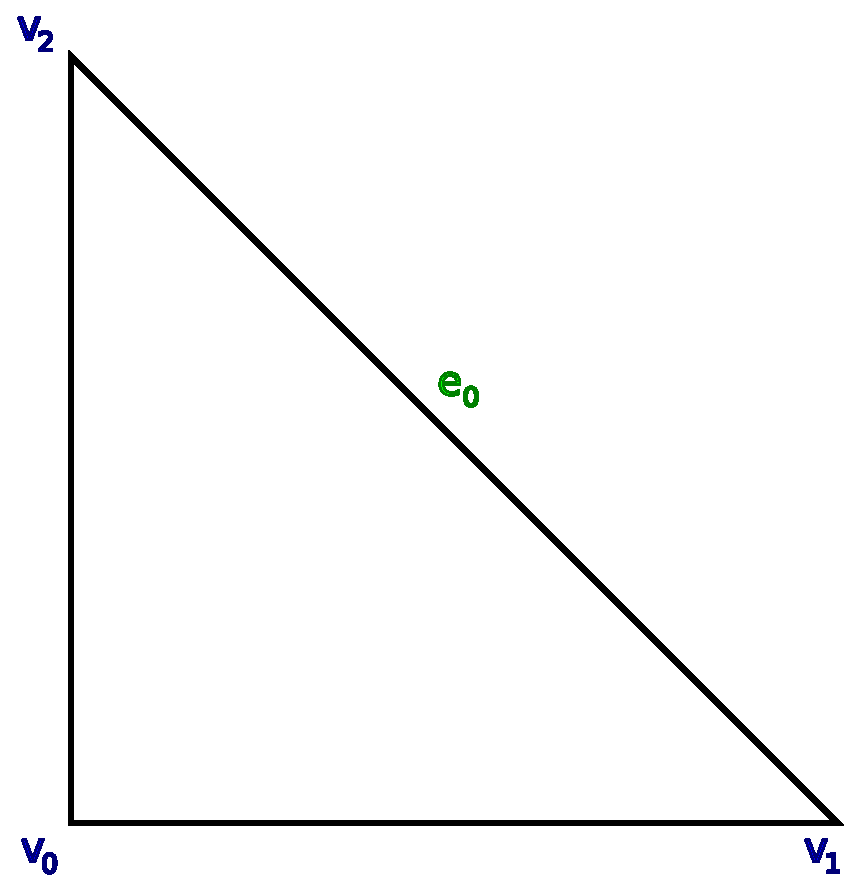
\includegraphics[width=5cm]{eps/ordering_example_triangle.eps}
    \caption{Entities are ordered based on a lexicographical ordering
      of their non-incident vertices. The first edge $e_0$ is non-incident
      with vertex $v_0$.}
    \label{fig:orderingexample,triangle}
  \end{center}
\end{figure}

\begin{figure}[H]
  \begin{center}
    \psfrag{v0}{$v_0$}
    \psfrag{v1}{$v_1$}
    \psfrag{v2}{$v_2$}
    \psfrag{v3}{$v_3$}
    \psfrag{e0}{$e_0$}
    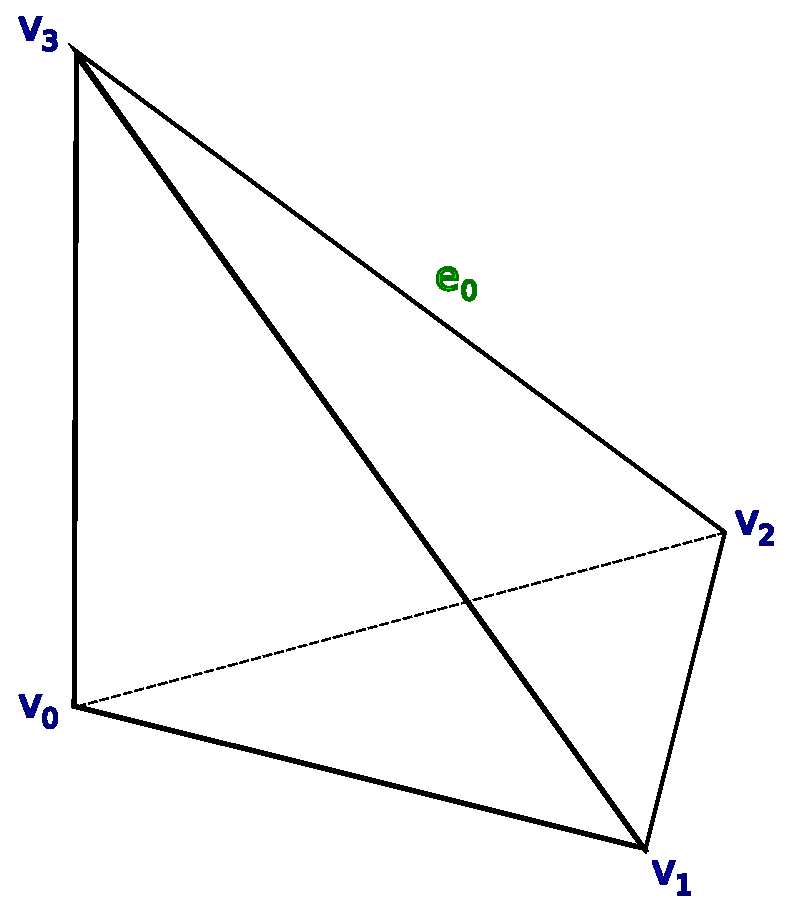
\includegraphics[width=7cm]{eps/ordering_example_tetrahedron.eps}
    \caption{Entities are ordered based on a lexicographical ordering
      of their non-incident vertices. The first edge $e_0$ is non-incident
      with vertices $v_0$ and $v_1$.}
    \label{fig:orderingexample,tetrahedron}
  \end{center}
\end{figure}

\subsection{Limitations}

The UFC specification is only concerned with the ordering of mesh
entities with respect to cells, not the ordering of mesh entities
with respect to other mesh entities of lower dimension. In other
words, the UFC specification is only concerned with the ordering of
incidence relations of the class $d - d'$ where $d$ is the
topological dimension of the mesh and $d' < d$. For example, the UFC
specification is not concerned with the ordering of incidence
relations of the class $1 - 0$, that is, the ordering of vertices on
an edge, or incidence relations of the class $2 - 1$, that is, the
ordering of edges on a face.

\newpage
\section{The reference interval}

The reference interval is shown in Figure~\ref{fig:interval} and is
defined by its two vertices with coordinates as specified in
Table~\ref{tab:interval,vertices} and mesh entities as specified in
Table~\ref{tab:interval,entities}.

\begin{figure}[H]
  \begin{center}
    \psfrag{0}{$0$}
    \psfrag{1}{$1$}
    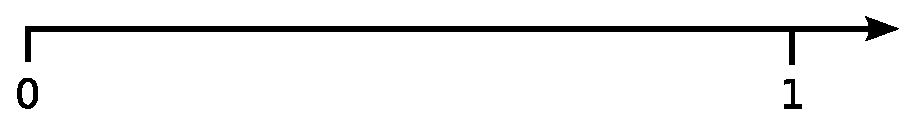
\includegraphics[width=10cm]{eps/interval.eps}
    \caption{The reference interval.}
    \label{fig:interval}
  \end{center}
\end{figure}

\begin{table}[H]
\linespread{1.2}\selectfont
  \begin{center}
    \begin{tabular}{|c|c|}
      \hline
      Vertex & Coordinate \\
      \hline
      \hline
      $v_0$ & $x = 0$ \\
      \hline
      $v_1$ & $x = 1$ \\
      \hline
    \end{tabular}
    \caption{Vertex coordinates of the reference interval.}
    \label{tab:interval,vertices}
  \end{center}
\end{table}

\begin{table}[H]
\linespread{1.2}\selectfont
  \begin{center}
    \begin{tabular}{|c|c|c|}
      \hline
      Entity & Incident vertices & Non-incident vertices \\
      \hline
      \hline
      $v_0 = (0, 0)$ & $\{v_0\}$ & $\{v_1\}$ \\
      \hline
      $v_1 = (0, 1)$ & $\{v_1\}$ & $\{v_0\}$ \\
      \hline
      $c_0 = (1, 0)$ & $\{v_0, v_1\}$ & $\emptyset$ \\
      \hline
    \end{tabular}
    \caption{Mesh entities of the reference interval.}
    \label{tab:interval,entities}
  \end{center}
\end{table}

\newpage
\section{The reference triangle}

The reference triangle is shown in Figure~\ref{fig:triangle} and is
defined by its three vertices with coordinates as specified in
Table~\ref{tab:triangle,vertices} and mesh entities as specified in
Table~\ref{tab:triangle,entities}.

\begin{figure}[H]
  \begin{center}
    \psfrag{v0}{$(0, 0)$}
    \psfrag{v1}{$(1, 0)$}
    \psfrag{v2}{$(0, 1)$}
    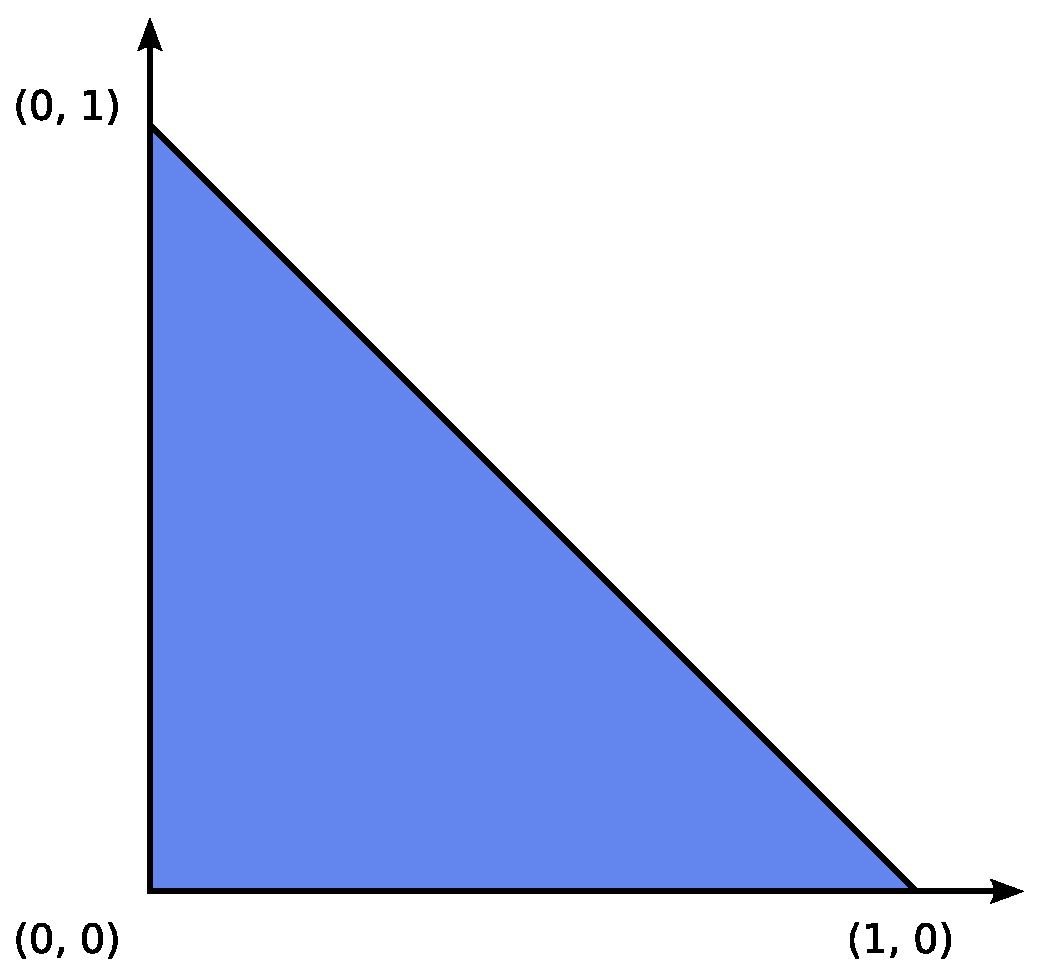
\includegraphics[width=10cm]{eps/triangle.eps}
    \caption{The reference triangle.}
    \label{fig:triangle}
  \end{center}
\end{figure}

\begin{table}[H]
\linespread{1.2}\selectfont
  \begin{center}
    \begin{tabular}{|c|c|}
      \hline
      Vertex & Coordinate \\
      \hline
      \hline
      $v_0 = (0, 0)$ & $x = (0, 0)$ \\
      \hline
      $v_1 = (0, 1)$ & $x = (1, 0)$ \\
      \hline
      $v_2 = (0, 2)$ & $x = (0, 1)$ \\
      \hline
    \end{tabular}
    \caption{Vertex coordinates of the reference triangle.}
    \label{tab:triangle,vertices}
  \end{center}
\end{table}

\begin{table}[H]
\linespread{1.2}\selectfont
  \begin{center}
    \begin{tabular}{|c|c|c|}
      \hline
      Entity & Incident vertices & Non-incident vertices \\
      \hline
      \hline
      $v_0 = (0, 0)$ & $\{v_0\}$ & $\{v_1, v_2\}$ \\
      \hline
      $v_1 = (0, 1)$ & $\{v_1\}$ & $\{v_0, v_2\}$ \\
      \hline
      $v_2 = (0, 2)$ & $\{v_2\}$ & $\{v_0, v_1\}$ \\
      \hline
      $e_0 = (1, 0)$ & $\{v_1, v_2\}$ & $\{v_0\}$ \\
      \hline
      $e_1 = (1, 1)$ & $\{v_0, v_2\}$ & $\{v_1\}$ \\
      \hline
      $e_2 = (1, 2)$ & $\{v_0, v_1\}$ & $\{v_2\}$ \\
      \hline
      $c_0 = (2, 0)$ & $\{v_0, v_1, v_2\}$ & $\emptyset$ \\
      \hline
    \end{tabular}
    \caption{Mesh entities of the reference triangle.}
    \label{tab:triangle,entities}
  \end{center}
\end{table}

\newpage
\section{The reference quadrilateral}

The reference quadrilateral is shown in Figure~\ref{fig:quadrilateral}
and is defined by its four vertices with coordinates as specified in
Table~\ref{tab:quadrilateral,vertices} and mesh entities as specified
in Table~\ref{tab:quadrilateral,entities}.

\begin{figure}[H]
  \begin{center}
    \psfrag{v0}{$(0, 0)$}
    \psfrag{v1}{$(1, 0)$}
    \psfrag{v2}{$(1, 1)$}
    \psfrag{v3}{$(0, 1)$}
    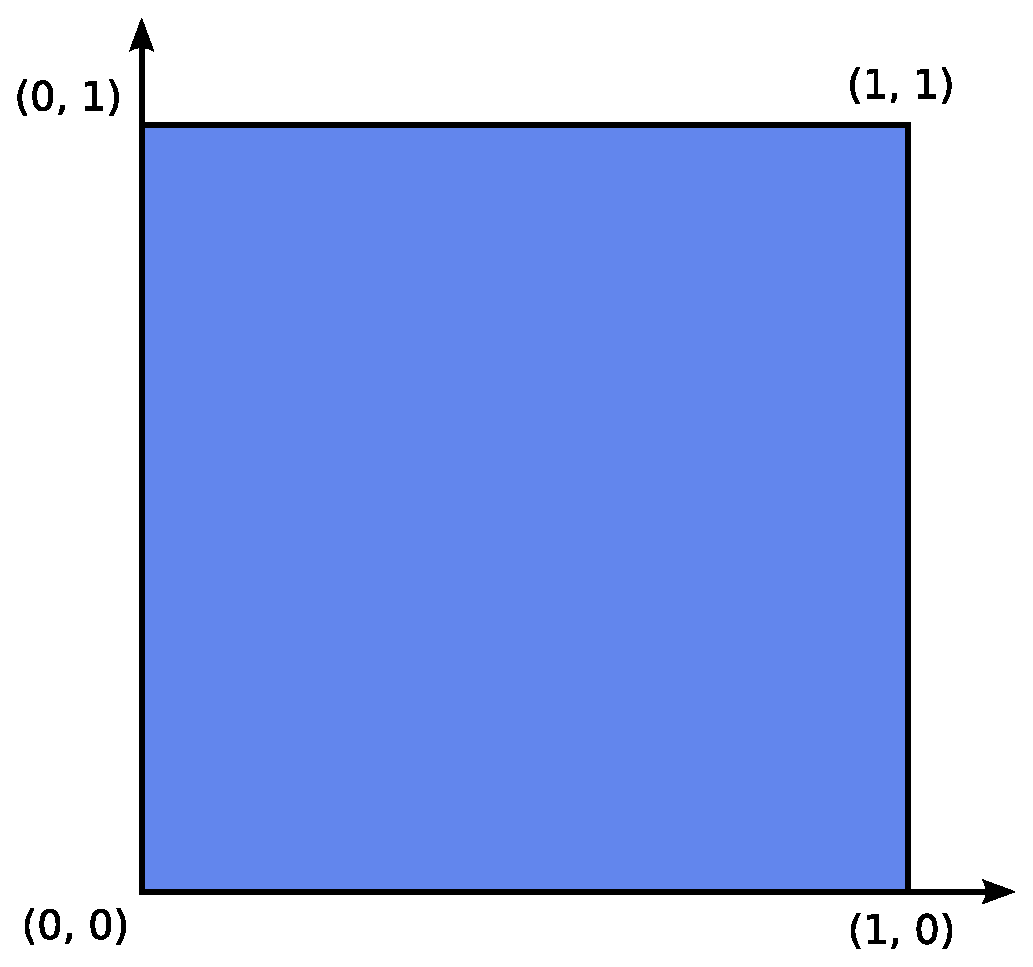
\includegraphics[width=10cm]{eps/quadrilateral.eps}
    \caption{The reference quadrilateral.}
    \label{fig:quadrilateral}
  \end{center}
\end{figure}

\begin{table}[H]
\linespread{1.2}\selectfont
  \begin{center}
    \begin{tabular}{|c|c|}
      \hline
      Vertex & Coordinate \\
      \hline
      \hline
      $v_0$ & $x = (0, 0)$ \\
      \hline
      $v_1$ & $x = (1, 0)$ \\
      \hline
      $v_2$ & $x = (1, 1)$ \\
      \hline
      $v_3$ & $x = (0, 1)$ \\
      \hline
    \end{tabular}
    \caption{Vertex coordinates of the reference quadrilateral.}
    \label{tab:quadrilateral,vertices}
  \end{center}
\end{table}

\begin{table}[H]
\linespread{1.2}\selectfont
  \begin{center}
    \begin{tabular}{|c|c|c|}
      \hline
      Entity & Incident vertices & Non-incident vertices \\
      \hline
      \hline
      $v_0 = (0, 0)$ & $\{v_0\}$ & $\{v_1, v_2, v_3\}$ \\
      \hline
      $v_1 = (0, 1)$ & $\{v_1\}$ & $\{v_0, v_2, v_3\}$ \\
      \hline
      $v_2 = (0, 2)$ & $\{v_2\}$ & $\{v_0, v_1, v_3\}$ \\
      \hline
      $v_3 = (0, 3)$ & $\{v_3\}$ & $\{v_0, v_1, v_2\}$ \\
      \hline
      $e_0 = (1, 0)$ & $\{v_2, v_3\}$ & $\{v_0, v_1\}$ \\
      \hline
      $e_1 = (1, 1)$ & $\{v_1, v_2\}$ & $\{v_0, v_3\}$ \\
      \hline
      $e_2 = (1, 2)$ & $\{v_0, v_3\}$ & $\{v_1, v_2\}$ \\
      \hline
      $e_3 = (1, 3)$ & $\{v_0, v_1\}$ & $\{v_2, v_3\}$ \\
      \hline
      $c_0 = (2, 0)$ & $\{v_0, v_1, v_2, v_3\}$ & $\emptyset$ \\
      \hline
    \end{tabular}
    \caption{Mesh entities of the reference quadrilateral.}
    \label{tab:quadrilateral,entities}
  \end{center}
\end{table}

\newpage
\section{The reference tetrahedron}

The reference tetrahedron is shown in Figure~\ref{fig:tetrahedron} and
is defined by its four vertices with coordinates as specified in
Table~\ref{tab:tetrahedron,vertices} and mesh entities as specified in
Table~\ref{tab:tetrahedron,entities}.

\begin{figure}[H]
  \begin{center}
    \psfrag{v0}{$(0, 0, 0)$}
    \psfrag{v1}{$(1, 0, 0)$}
    \psfrag{v2}{$(0, 1, 0)$}
    \psfrag{v3}{$(0, 0, 1)$}
    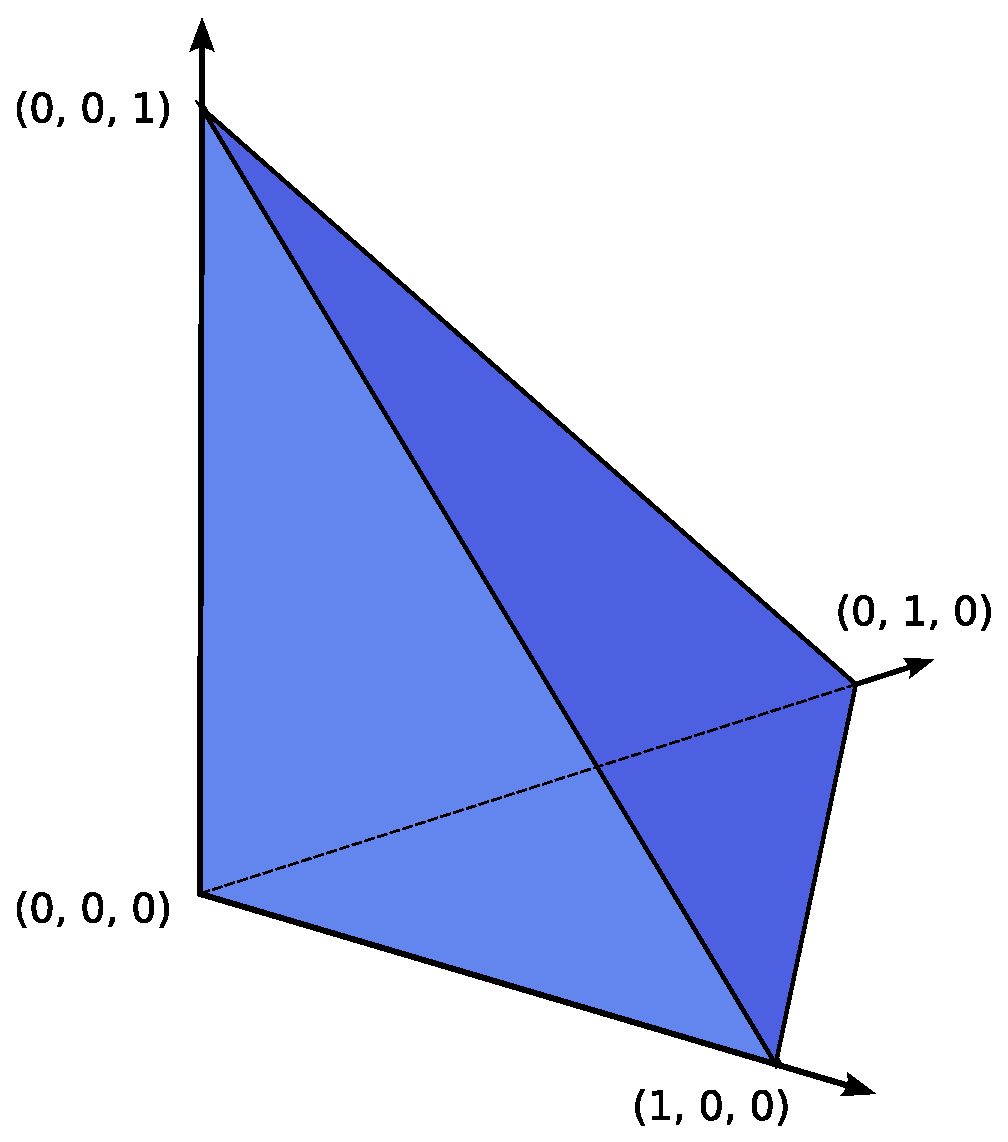
\includegraphics[width=10cm]{eps/tetrahedron.eps}
    \caption{The reference tetrahedron.}
    \label{fig:tetrahedron}
  \end{center}
\end{figure}

\begin{table}[H]
\linespread{1.2}\selectfont
  \begin{center}
    \begin{tabular}{|c|c|}
      \hline
      Vertex & Coordinate \\
      \hline
      \hline
      $v_0$ & $x = (0, 0, 0)$ \\
      \hline
      $v_1$ & $x = (1, 0, 0)$ \\
      \hline
      $v_2$ & $x = (0, 1, 0)$ \\
      \hline
      $v_3$ & $x = (0, 0, 1)$ \\
      \hline
    \end{tabular}
    \caption{Vertex coordinates of the reference tetrahedron.}
    \label{tab:tetrahedron,vertices}
  \end{center}
\end{table}

\begin{table}[H]
\linespread{1.2}\selectfont
  \begin{center}
    \begin{tabular}{|c|c|c|}
      \hline
      Entity & Incident vertices & Non-incident vertices \\
      \hline
      \hline
      $v_0 = (0, 0)$ & $\{v_0\}$ & $\{v_1, v_2, v_3\}$ \\
      \hline
      $v_1 = (0, 1)$ & $\{v_1\}$ & $\{v_0, v_2, v_3\}$ \\
      \hline
      $v_2 = (0, 2)$ & $\{v_2\}$ & $\{v_0, v_1, v_3\}$ \\
      \hline
      $v_3 = (0, 3)$ & $\{v_3\}$ & $\{v_0, v_1, v_2\}$ \\
      \hline
      $e_0 = (1, 0)$ & $\{v_2, v_3\}$ & $\{v_0, v_1\}$ \\
      \hline
      $e_1 = (1, 1)$ & $\{v_1, v_3\}$ & $\{v_0, v_2\}$ \\
      \hline
      $e_2 = (1, 2)$ & $\{v_1, v_2\}$ & $\{v_0, v_3\}$ \\
      \hline
      $e_3 = (1, 3)$ & $\{v_0, v_3\}$ & $\{v_1, v_2\}$ \\
      \hline
      $e_4 = (1, 4)$ & $\{v_0, v_2\}$ & $\{v_1, v_3\}$ \\
      \hline
      $e_5 = (1, 5)$ & $\{v_0, v_1\}$ & $\{v_2, v_3\}$ \\
      \hline
      $f_0 = (2, 0)$ & $\{v_1, v_2, v_3\}$ & $\{v_0\}$ \\
      \hline
      $f_1 = (2, 1)$ & $\{v_0, v_2, v_3\}$ & $\{v_1\}$ \\
      \hline
      $f_2 = (2, 2)$ & $\{v_0, v_1, v_3\}$ & $\{v_2\}$ \\
      \hline
      $f_3 = (2, 3)$ & $\{v_0, v_1, v_2\}$ & $\{v_3\}$ \\
      \hline
      $c_0 = (3, 0)$ & $\{v_0, v_1, v_2, v_3\}$ & $\emptyset$ \\
      \hline
    \end{tabular}
    \caption{Mesh entities of the reference tetrahedron.}
        \label{tab:tetrahedron,entities} 
  \end{center}
\end{table}

\newpage
\section{The reference hexahedron}

The reference hexahedron is shown in Figure~\ref{fig:hexahedron} and
is defined by its eight vertices with coordinates as specified in
Table~\ref{tab:hexahedron,vertices} and mesh entities as specified in
Table~\ref{tab:hexahedron,entities}.

\begin{figure}[H]
\linespread{1.2}\selectfont
  \begin{center}
    \psfrag{v0}{$(0, 0, 0)$}
    \psfrag{v1}{$(1, 0, 0)$}
    \psfrag{v2}{$(1, 1, 0)$}
    \psfrag{v3}{$(0, 1, 0)$}
    \psfrag{v4}{$(0, 0, 1)$}
    \psfrag{v5}{$(1, 0, 1)$}
    \psfrag{v6}{$(1, 1, 1)$}
    \psfrag{v7}{$(0, 1, 1)$}
    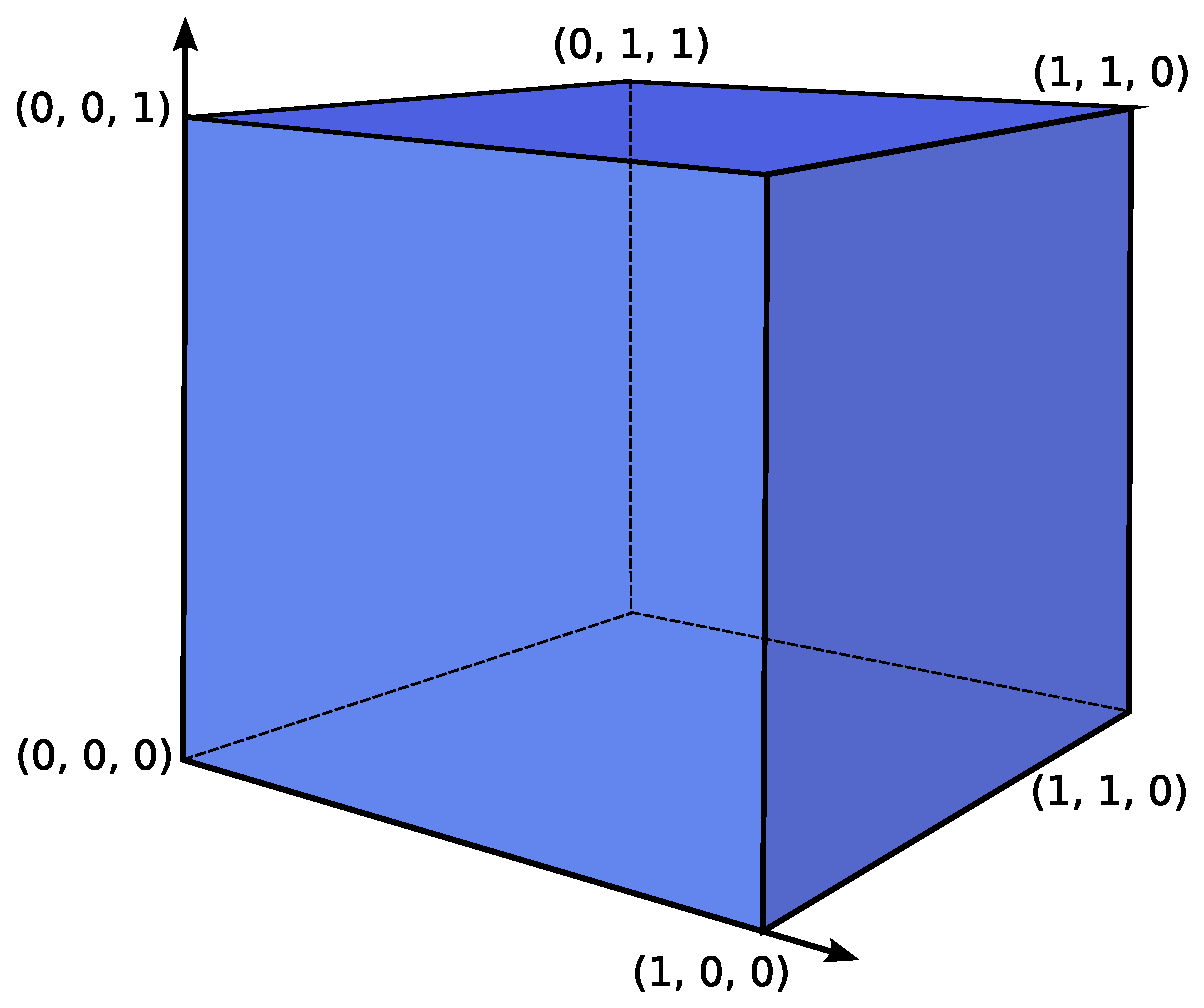
\includegraphics[width=10cm]{eps/hexahedron.eps}
    \caption{The reference hexahedron.}
    \label{fig:hexahedron}
  \end{center}
\end{figure}

\begin{table}[H]
\linespread{1.2}\selectfont
  \begin{center}
    \begin{tabular}{|c|c|}
      \hline
      Vertex & Coordinate \\
      \hline
      \hline
      $v_0$ & $x = (0, 0, 0)$ \\
      \hline
      $v_1$ & $x = (1, 0, 0)$ \\
      \hline
      $v_2$ & $x = (1, 1, 0)$ \\
      \hline
      $v_3$ & $x = (0, 1, 0)$ \\
      \hline
      $v_4$ & $x = (0, 0, 1)$ \\
      \hline
      $v_5$ & $x = (1, 0, 1)$ \\
      \hline
      $v_6$ & $x = (1, 1, 1)$ \\
      \hline
      $v_7$ & $x = (0, 1, 1)$ \\
      \hline
    \end{tabular}
    \caption{Vertex coordinates of the reference hexahedron.}
    \label{tab:hexahedron,vertices}
  \end{center}
\end{table}

\begin{table}[H]
\linespread{1.2}\selectfont
  \begin{center}
    \begin{tabular}{|c|c|c|}
      \hline
      Entity & Incident vertices & Non-incident vertices \\
      \hline
      \hline
      $v_0 = (0, 0)$ & $\{v_0\}$ & $\{v_1, v_2, v_3, v_4, v_5, v_6, v_7\}$ \\
      \hline
      $v_1 = (0, 1)$ & $\{v_1\}$ & $\{v_0, v_2, v_3, v_4, v_5, v_6, v_7\}$ \\
      \hline
      $v_2 = (0, 2)$ & $\{v_2\}$ & $\{v_0, v_1, v_3, v_4, v_5, v_6, v_7\}$ \\
      \hline
      $v_3 = (0, 3)$ & $\{v_3\}$ & $\{v_0, v_1, v_2, v_4, v_5, v_6, v_7\}$ \\
      \hline
      $v_4 = (0, 4)$ & $\{v_4\}$ & $\{v_0, v_1, v_2, v_3, v_5, v_6, v_7\}$ \\
      \hline
      $v_5 = (0, 5)$ & $\{v_5\}$ & $\{v_0, v_1, v_2, v_3, v_4, v_6, v_7\}$ \\
      \hline
      $v_6 = (0, 6)$ & $\{v_6\}$ & $\{v_0, v_1, v_2, v_3, v_4, v_5, v_7\}$ \\
      \hline
      $v_7 = (0, 7)$ & $\{v_7\}$ & $\{v_0, v_1, v_2, v_3, v_4, v_5, v_6\}$ \\
      \hline
      $e_0 = (1, 0)$ & $\{v_6, v_7\}$ & $\{v_0, v_1, v_2, v_3, v_4, v_5\}$ \\
      \hline
      $e_1 = (1, 1)$ & $\{v_5, v_6\}$ & $\{v_0, v_1, v_2, v_3, v_4, v_7\}$ \\
      \hline
      $e_2 = (1, 2)$ & $\{v_4, v_7\}$ & $\{v_0, v_1, v_2, v_3, v_5, v_6\}$ \\
      \hline
      $e_3 = (1, 3)$ & $\{v_4, v_5\}$ & $\{v_0, v_1, v_2, v_3, v_6, v_7\}$ \\
      \hline
      $e_4 = (1, 4)$ & $\{v_3, v_7\}$ & $\{v_0, v_1, v_2, v_4, v_5, v_6\}$ \\
      \hline
      $e_5 = (1, 5)$ & $\{v_2, v_6\}$ & $\{v_0, v_1, v_3, v_4, v_5, v_7\}$ \\
      \hline
      $e_6 = (1, 6)$ & $\{v_2, v_3\}$ & $\{v_0, v_1, v_4, v_5, v_6, v_7\}$ \\
      \hline
      $e_7 = (1, 7)$ & $\{v_1, v_5\}$ & $\{v_0, v_2, v_3, v_4, v_6, v_7\}$ \\
      \hline
      $e_8 = (1, 8)$ & $\{v_1, v_2\}$ & $\{v_0, v_3, v_4, v_5, v_6, v_7\}$ \\
      \hline
      $e_9 = (1, 9)$ & $\{v_0, v_4\}$ & $\{v_1, v_2, v_3, v_5, v_6, v_7\}$ \\
      \hline
      $e_{10} = (1, 10)$ & $\{v_0, v_3\}$ & $\{v_1, v_2, v_4, v_5, v_6, v_7\}$ \\
      \hline
      $e_{11} = (1, 11)$ & $\{v_0, v_1\}$ & $\{v_2, v_3, v_4, v_5, v_6, v_7\}$ \\
      \hline
      $f_0 = (2, 0)$ & $\{v_4, v_5, v_6, v_7\}$ & $\{v_0, v_1, v_2, v_3\}$ \\
      \hline
      $f_1 = (2, 1)$ & $\{v_2, v_3, v_6, v_7\}$ & $\{v_0, v_1, v_4, v_5\}$ \\
      \hline
      $f_2 = (2, 2)$ & $\{v_1, v_2, v_5, v_6\}$ & $\{v_0, v_3, v_4, v_7\}$ \\
      \hline
      $f_3 = (2, 3)$ & $\{v_0, v_3, v_4, v_7\}$ & $\{v_1, v_2, v_5, v_6\}$ \\
      \hline
      $f_4 = (2, 4)$ & $\{v_0, v_1, v_4, v_5\}$ & $\{v_2, v_3, v_6, v_7\}$ \\
      \hline
      $f_5 = (2, 5)$ & $\{v_0, v_1, v_2, v_3\}$ & $\{v_4, v_5, v_6, v_7\}$ \\
      \hline
      $c_0 = (3, 0)$ & $\{v_0, v_1, v_2, v_3, v_4, v_5, v_6, v_7\}$ & $\emptyset$ \\
      \hline
    \end{tabular}
    \caption{Mesh entities of the reference hexahedron.}
    \label{tab:hexahedron,entities}
  \end{center}
\end{table}
